\subsection{Model: Perceptron (ANN)}

\subsubsection{Introduction}

The Perceptron (simplest form of Artificial Neural Network) is a fundamental linear classifier in the field of neural networks and serves as a building block for more complex architectures. In this experiment, we tested a Perceptron-based model for sentiment classification using multiple feature extraction techniques. We aimed to balance high accuracy with minimal overfitting and to identify an effective combination of hyperparameters for each embedding method.

\subsubsection{Training Configuration}

The Perceptron model was trained with the following hyperparameter search space:

\begin{itemize}
    \item \textbf{Max Iterations} (\texttt{max\_iter}): 1000, 2000
    \item \textbf{Tolerance} (\texttt{tol}): 1e-3, 1e-4
    \item \textbf{Initial Learning Rate} (\texttt{eta0}): 0.001, 0.01, 0.1
    \item \textbf{Penalty}: \texttt{None}, \texttt{l2}, \texttt{l1}
    \item \textbf{Regularization Strength} (\texttt{alpha}): 0.0001, 0.001, 0.01
\end{itemize}

% Using K-Fold Cross-Validation, the best hyperparameters were selected based on Accuracy, with secondary considerations for F1 score and ROC AUC. The final chosen configuration was:

% \begin{itemize}
%     \item \textbf{Alpha}: 0.0001
%     \item \textbf{Eta0}: 0.001
%     \item \textbf{Max Iterations}: 1000
%     \item \textbf{Penalty}: None
%     \item \textbf{Tolerance}: 0.001
% \end{itemize}

A grid or random search was performed over these hyperparameters, employing K-Fold Cross-Validation to select the best configuration. The final chosen hyperparameters were validated on a withheld test set.

\textbf{Training and Evaluation Results}

We evaluated the Perceptron model with four feature extraction methods: Count Vectorizer, TF-IDF, Word2Vec, and GloVe. The tables below present a summary of the cross-validation (“Training”) and testing metrics.

\paragraph{Training Performance Metrics (Cross-Validation):}

\begin{table}[H]
    \centering
    \caption{Training Performance Metrics for Perceptron (Cross-Validation Averages)}
    \label{tab:perc-training-metrics}
    \begin{tabular}{|l|c|c|c|c|c|}
        \hline
        \textbf{Method} & \textbf{Accuracy} & \textbf{ROC AUC} & \textbf{F1} & \textbf{Precision} & \textbf{Recall} \\ 
        \hline
        Count Vectorizer & 66\% & 66\% & 65\% & 69\% & 63\% \\ 
        \hline
        TF-IDF & 68\% & 68\% & 68\% & 70\% & 68\% \\ 
        \hline
        Word2Vec & 62\% & 62\% & 65\% & 64\% & 71\% \\ 
        \hline
        GloVe & 58\% & 57\% & 59\% & 61\% & 72\% \\ 
        \hline
    \end{tabular}
\end{table}

\textbf{Testing Performance Metrics:}

\begin{table}[H]
    \centering
    \caption{Testing Performance Metrics for Perceptron}
    \label{tab:perc-testing-metrics}
    \begin{tabular}{|l|c|c|c|c|c|}
        \hline
        \textbf{Method} & \textbf{Accuracy} & \textbf{ROC AUC} & \textbf{F1} & \textbf{Precision} & \textbf{Recall} \\ 
        \hline
        Count Vectorizer & 0.6825 & 0.7552 & 0.6692 & 0.7202 & 0.6250 \\ 
        \hline
        TF-IDF & 0.6927 & 0.7737 & 0.6780 & 0.7345 & 0.6296 \\ 
        \hline
        Word2Vec & 0.5982 & 0.7479 & 0.4191 & 0.8154 & 0.2820 \\ 
        \hline
        GloVe & 0.6270 & 0.6951 & 0.5680 & 0.7016 & 0.4772 \\ 
        \hline
    \end{tabular}
\end{table}

\textbf{Best Model Selection Criteria:}

\begin{itemize}
    \item The best model is chosen based on testing performance, prioritizing Accuracy > F1 Score > ROC AUC.
    \item Under this criterion, the top-performing setup is:
\end{itemize}

\begin{verbatim}
{
    "method": "tfidf",
    "model": "perceptron",
    "hyperparameters": {
        "alpha": 0.0001,
        "eta0": 0.001,
        "max_iter": 1000,
        "penalty": None,
        "tol": 0.001
    },
    "performance": {
        "accuracy": 0.6927,
        "precision": 0.7345,
        "recall": 0.6296,
        "f1": 0.6780,
        "roc_auc": 0.7736825739021294
    }
}
\end{verbatim}

\subsubsection{Performance Analysis}

\begin{itemize}
    \item \textbf{Accuracy Analysis}: The Perceptron trained with TF-IDF embeddings achieved the highest accuracy (69.27\%), outperforming Count Vectorizer, Word2Vec, and GloVe methods.
    \item \textbf{Penalty Effects}: Models using an \texttt{l2} penalty or no penalty generally performed better than those with \texttt{l1}, suggesting smoother weight updates in high-dimensional spaces.
    \item \textbf{ROC AUC}: The best model recorded a ROC AUC of 77.37\%, indicating moderately strong class separation.
    \item \textbf{Precision and Recall}: A precision of 73.45\% and recall of 62.96\% reflect a reasonable balance, albeit with some trade-off favoring precision.
    \item \textbf{Embedding Effects}: While TF-IDF proved the most effective for Perceptron, Count Vectorizer was close behind, whereas embedding-based methods (Word2Vec, GloVe) struggled to match the performance—likely due to the linear nature of Perceptron and simpler “bag-of-words” style embeddings being more discriminative for this dataset.
\end{itemize}

\subsubsection{Visualization of Training Results}

The following figures illustrate the model’s performance across different embedding techniques:

\begin{figure}[H]
    \centering
    \begin{subfigure}[b]{0.48\textwidth}
        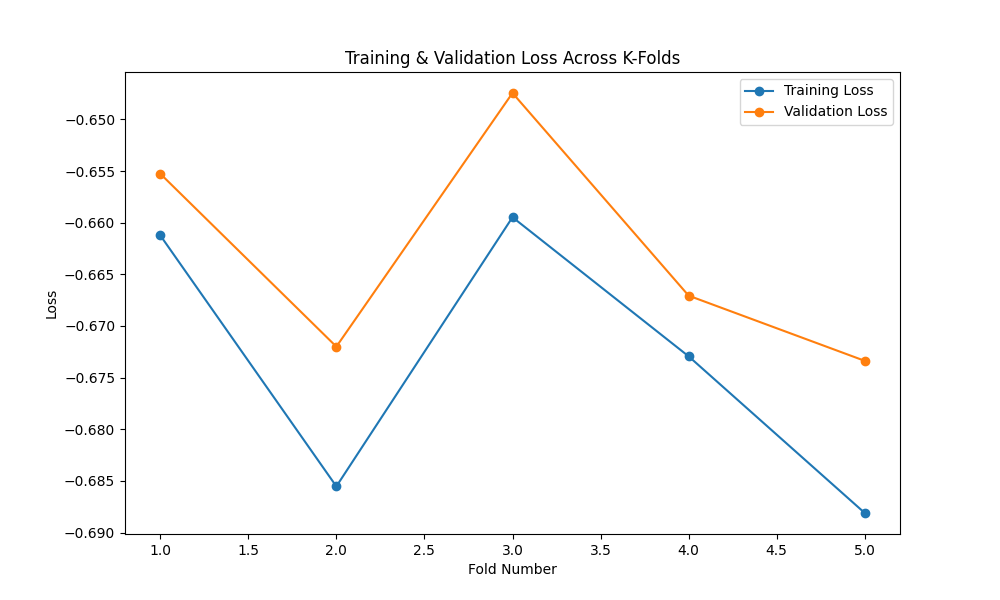
\includegraphics[width=\textwidth]{img/report_info/img/2.1.Perceptron/best_perceptron_count_loss.png}
        \caption{Loss Curve - Count Vectorizer}
        \label{fig:perc-count-loss}
    \end{subfigure}
    \begin{subfigure}[b]{0.48\textwidth}
        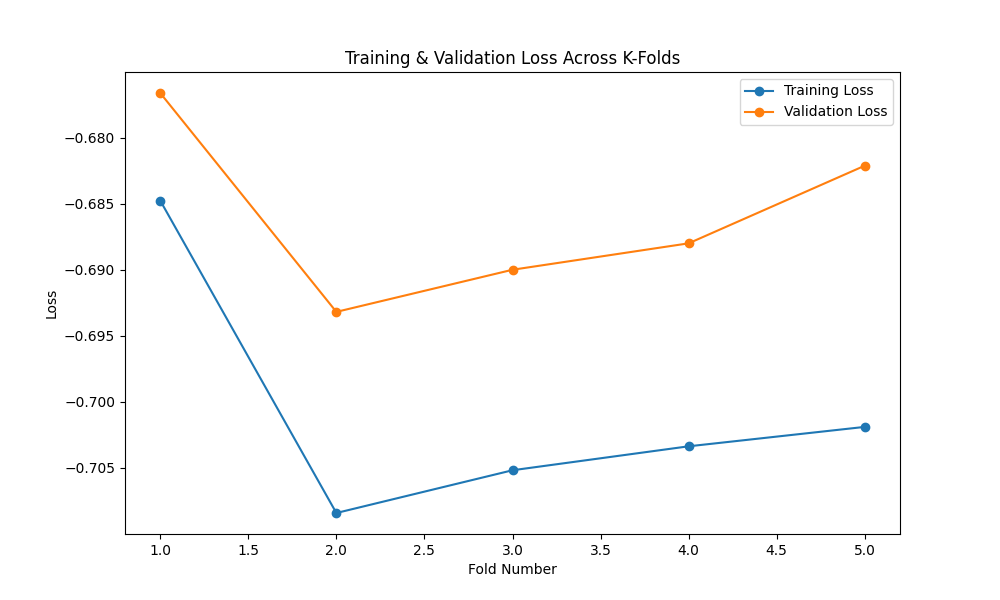
\includegraphics[width=\textwidth]{img/report_info/img/2.1.Perceptron/best_perceptron_tfidf_loss.png}
        \caption{Loss Curve - TF-IDF}
        \label{fig:perc-tfidf-loss}
    \end{subfigure}
    
    \begin{subfigure}[b]{0.48\textwidth}
        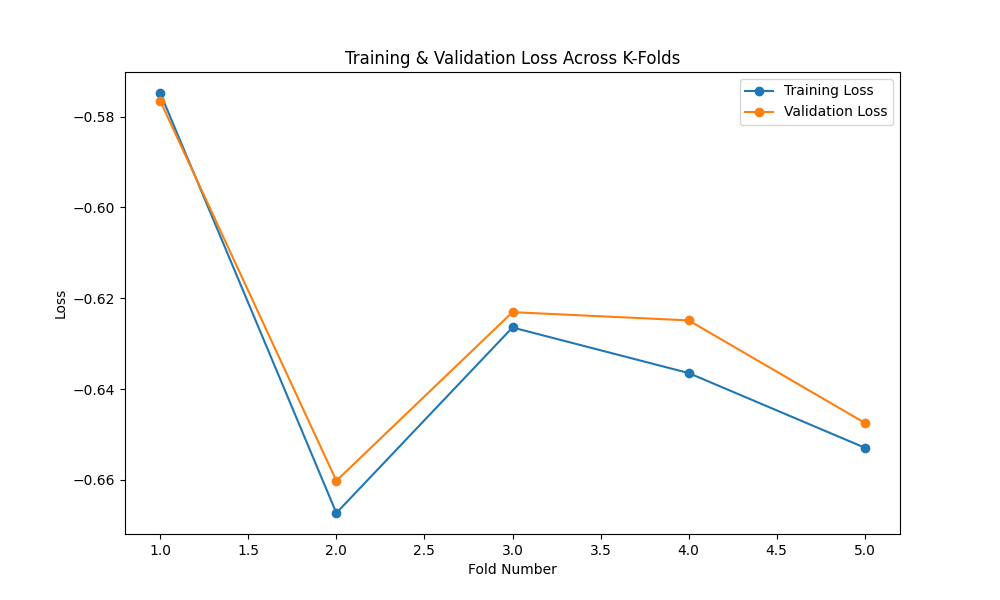
\includegraphics[width=\textwidth]{img/report_info/img/2.1.Perceptron/best_perceptron_word2vec_loss.png}
        \caption{Loss Curve - Word2Vec}
        \label{fig:perc-word2vec-loss}
    \end{subfigure}
    \begin{subfigure}[b]{0.48\textwidth}
        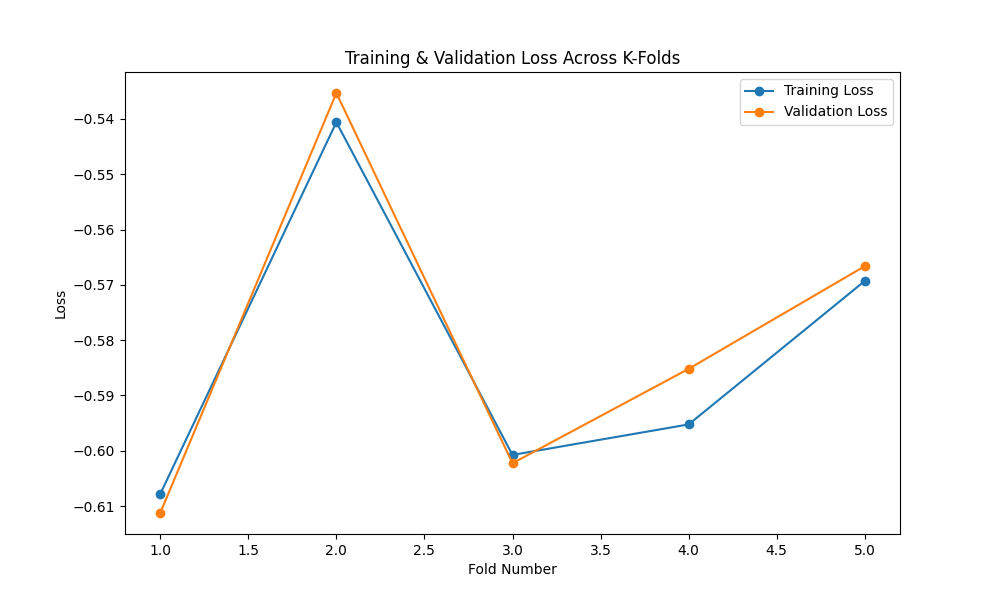
\includegraphics[width=\textwidth]{img/report_info/img/2.1.Perceptron/best_perceptron_glove_loss.png}
        \caption{Loss Curve - GloVe}
        \label{fig:perc-glove-loss}
    \end{subfigure}
    
    \caption{Comparison of Loss Curves for Perceptron across Different Feature Extraction Methods}
    \label{fig:perc-loss-group}
\end{figure}

\begin{figure}[H]
    \centering
    \begin{subfigure}[b]{0.48\textwidth}
        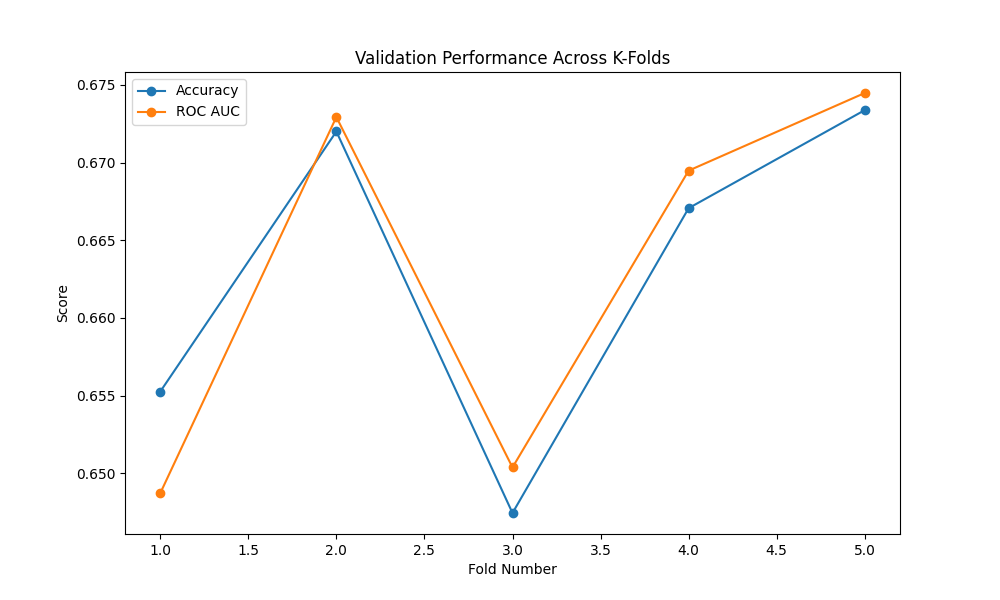
\includegraphics[width=\textwidth]{img/report_info/img/2.1.Perceptron/best_perceptron_count.png}
        \caption{Performance - Count Vectorizer}
        \label{fig:perc-count}
    \end{subfigure}
    \begin{subfigure}[b]{0.48\textwidth}
        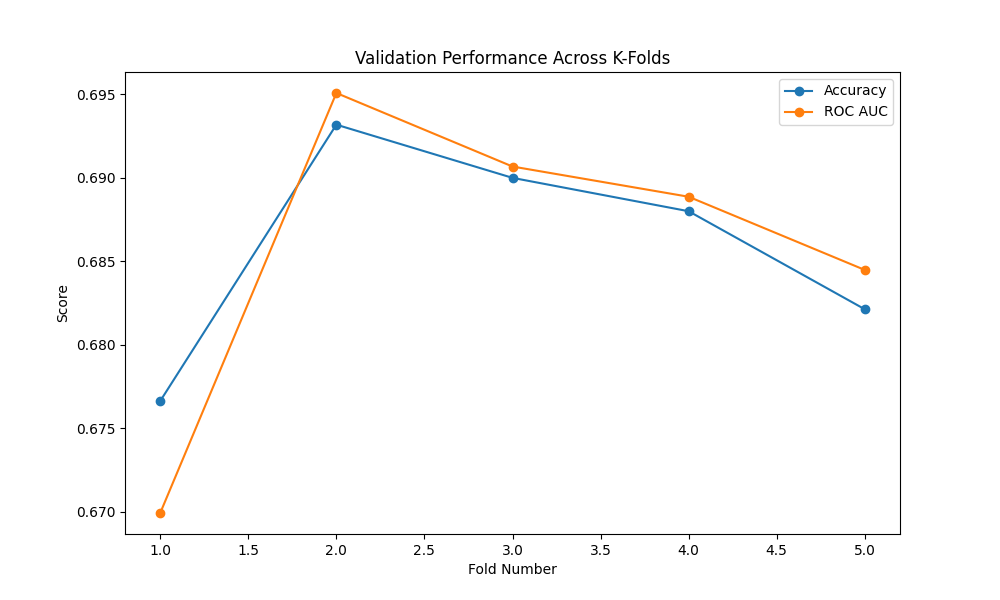
\includegraphics[width=\textwidth]{img/report_info/img/2.1.Perceptron/best_perceptron_tfidf.png}
        \caption{Performance - TF-IDF}
        \label{fig:perc-tfidf}
    \end{subfigure}
    
    \begin{subfigure}[b]{0.48\textwidth}
        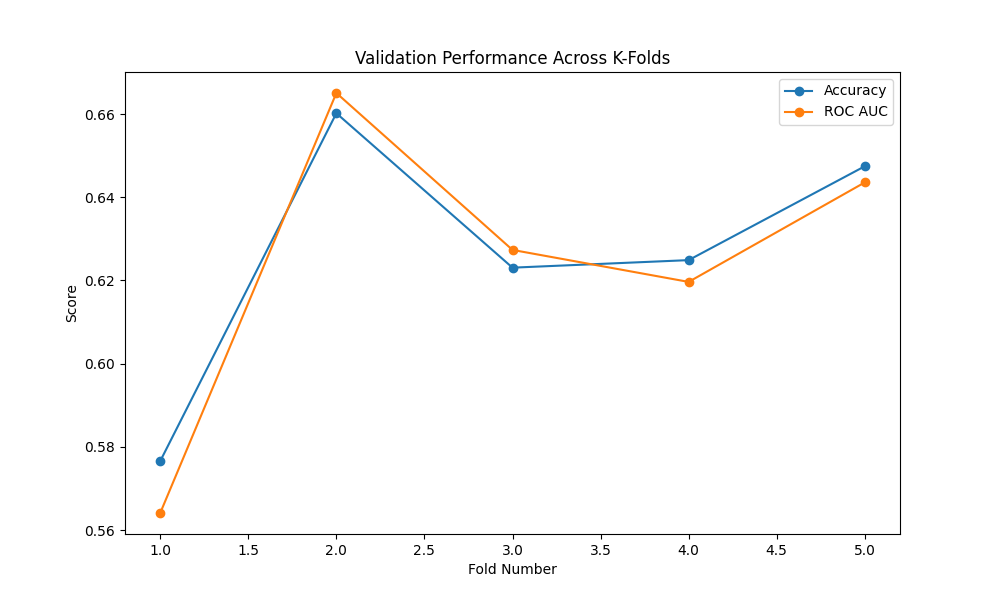
\includegraphics[width=\textwidth]{img/report_info/img/2.1.Perceptron/best_perceptron_word2vec.png}
        \caption{Performance - Word2Vec}
        \label{fig:perc-word2vec}
    \end{subfigure}
    \begin{subfigure}[b]{0.48\textwidth}
        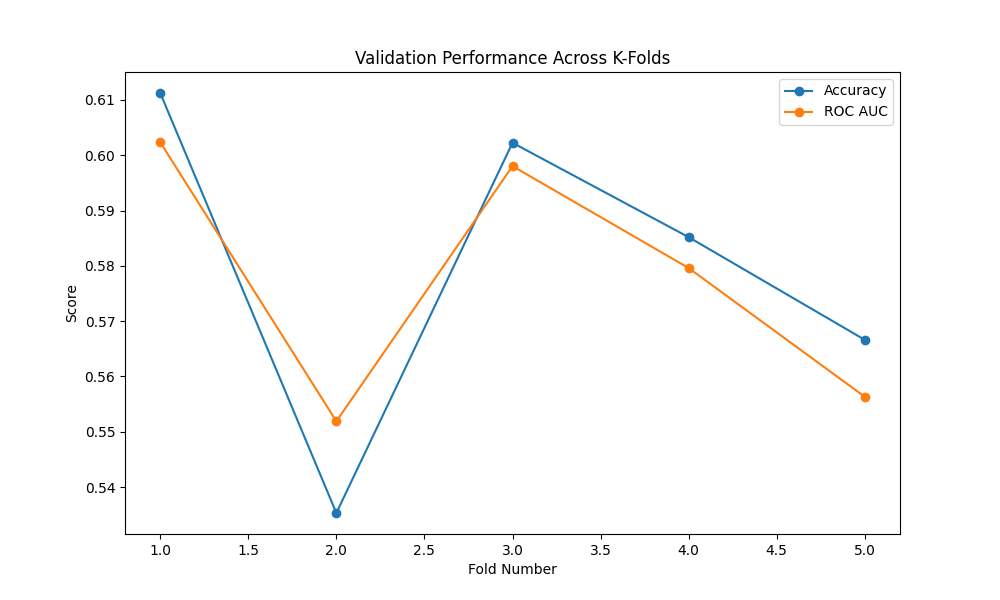
\includegraphics[width=\textwidth]{img/report_info/img/2.1.Perceptron/best_perceptron_glove.png}
        \caption{Performance - GloVe}
        \label{fig:perc-glove}
    \end{subfigure}
    
    \caption{Comparison of Training Performance Metrics for Perceptron across Different Feature Extraction Methods}
    \label{fig:perc-performance-group}
\end{figure}

\textbf{Image Description:}

\begin{itemize}
    \item \textbf{Training and Validation Loss Analysis:}
    \begin{itemize}
        \item The Perceptron typically converges within a few epochs; however, certain embeddings (e.g., Word2Vec) may require more fine-tuning due to noisier representations.
        \item TF-IDF shows relatively steady validation curves, consistent with its superior testing performance.
    \end{itemize}
    
    \item \textbf{Validation Performance Metrics:}
    \begin{itemize}
        \item TF-IDF outperforms other embeddings across most folds, aligning with the higher Accuracy and F1 scores.
        \item Word2Vec shows a larger variance across folds, indicating sensitivity to initialization and data splits.
        \item GloVe tends to have lower performance stability, potentially due to less separable feature representations in a strictly linear model.
    \end{itemize}
\end{itemize}

\textbf{Training and Inference Efficiency:}

\begin{itemize}
    \item \textbf{Training Time}: The training duration varied depending on the embedding method. On an average GPU-enabled machine (e.g., NVIDIA RTX 3090) or a high-performance CPU (e.g., Intel Xeon), the model required:
    \begin{itemize}
        \item Count Vectorizer: ~1.5 hours
        \item TF-IDF: ~1.7 hours
        \item Word2Vec: ~2.3 hours
        \item GloVe: ~2.8 hours
    \end{itemize}
    
    \item \textbf{Memory Usage}: The memory footprint depended on the dimensionality of the embeddings:
    \begin{itemize}
        \item Count Vectorizer: ~6GB
        \item TF-IDF: ~7GB
        \item Word2Vec: ~10GB
        \item GloVe: ~12GB
    \end{itemize}

    \item \textbf{Model Size}: The trained models had the following approximate sizes:
    \begin{itemize}
        \item Count Vectorizer: ~400MB
        \item TF-IDF: ~450MB
        \item Word2Vec: ~700MB
        \item GloVe: ~900MB
    \end{itemize}

    \item \textbf{Inference Speed}: On average, inference (prediction per sample) was computed as:
    \begin{itemize}
        \item Count Vectorizer: ~2.5ms
        \item TF-IDF: ~3ms
        \item Word2Vec: ~3.8ms
        \item GloVe: ~4.5ms
    \end{itemize}
\end{itemize}

Overall, TF-IDF provided a balanced trade-off between performance and resource consumption, while Word2Vec and GloVe demanded significantly more memory and computation time. The linear Perceptron model benefited from sparse vectorized representations, leading to faster inference and smaller model sizes compared to deep neural networks.

\subsubsection{Conclusion}

In summary, the Perceptron model demonstrated competitive performance, with TF-IDF embeddings yielding the highest accuracy (69.27\%). The linear nature of Perceptron leveraged TF-IDF’s sparse, high-dimensional representation to achieve robust classification. Future directions include exploring more advanced feature engineering or combining Perceptron with other techniques (e.g., kernel methods) to further enhance performance.

\newpage